\documentclass[aspectratio=169]{beamer}
% Shared preamble for ml/ slide decks.
% Each lecture .tex starts with:
%   \documentclass[aspectratio=169]{beamer}
%   % Shared preamble for ml/ slide decks.
% Each lecture .tex starts with:
%   \documentclass[aspectratio=169]{beamer}
%   % Shared preamble for ml/ slide decks.
% Each lecture .tex starts with:
%   \documentclass[aspectratio=169]{beamer}
%   \input{../preamble}
% Compile from inside the chapter folder so \input{../preamble} resolves.

\usetheme{default}
\usecolortheme{dove}

\setbeamertemplate{navigation symbols}{}
\setbeamertemplate{footline}{%
  \hfill{\large\insertframenumber\,/\,\inserttotalframenumber}\hspace{0.8em}\vspace{0.5em}%
}

% Project palette (existing, kept for backwards compatibility with deferred/*)
\definecolor{popblue}{RGB}{52, 101, 164}
\definecolor{sampred}{RGB}{204, 0, 0}
\definecolor{paramgreen}{RGB}{0, 140, 70}
\definecolor{warnred}{RGB}{180, 40, 40}
\definecolor{orange1}{RGB}{220, 120, 0}
\definecolor{violet1}{RGB}{120, 50, 160}
\definecolor{lightbg}{RGB}{245, 245, 250}

% Armenian flag palette (use these for any 3-color highlight; per CLAUDE.md).
% "Nice versions": slightly de-saturated from the official spec for slide use,
% so they don't burn out under projector colors. Originals kept as *_pure.
\definecolor{armred}{RGB}{200, 30, 40}      % nice red (official #D90012 muted)
\definecolor{armblue}{RGB}{30, 70, 160}     % nice blue (official #0033A0 muted)
\definecolor{armorange}{RGB}{230, 160, 30}  % nice orange (official #F2A800 muted)
\definecolor{armred_pure}{HTML}{D90012}     % official Armenian flag red
\definecolor{armblue_pure}{HTML}{0033A0}    % official Armenian flag blue
\definecolor{armorange_pure}{HTML}{F2A800}  % official Armenian flag orange

\setbeamercolor{frametitle}{fg=popblue}
\setbeamercolor{title}{fg=popblue}

\usepackage{pgfplots}
\usepackage{tikz}
\usetikzlibrary{shapes, arrows.meta, positioning, calc, decorations.pathreplacing, patterns, matrix}
\pgfplotsset{compat=1.18}
\usepackage{amsmath, amssymb, amsfonts}
\usepackage{bm}
\usepackage{dsfont}
\usepackage{array}
\usepackage{pifont}
\usepackage{colortbl}
\usepackage{fontenc}

% Callout boxes. Purely additive - existing decks are unaffected.
% Usage: \begin{tcolorbox}[colback=armblue!8, colframe=armblue, boxrule=0.6pt, arc=2pt,
%                          title=\textbf{Key idea}] ... \end{tcolorbox}
% Palette convention (ml/SLIDE_STYLE.md): armblue=key idea, armred=trap/warning,
% paramgreen=takeaway or "Next", armorange=watch-out.
\usepackage[most]{tcolorbox}

% Cleaner table rules (\toprule, \midrule, \bottomrule). Also purely additive.
\usepackage{booktabs}

% \cancel{...} for struck-through terms in derivations (added 2026-08-11 for the
% importance-sampling frame in ch11_rl, where the dynamics cancel). Purely additive.
\usepackage{cancel}

% Minimal ML notation macros (subset of slds-lmu latex-math/basic-ml.tex).
% Kept here so we don't have to inline-expand every \thetav, \xv, etc.
% when porting upstream slides.
\newcommand{\R}{\mathds{R}}
\newcommand{\N}{\mathds{N}}
\newcommand{\E}{\mathds{E}}
\newcommand{\Xspace}{\mathcal{X}}
\newcommand{\Yspace}{\mathcal{Y}}
\newcommand{\Hspace}{\mathcal{H}}
\newcommand{\D}{\mathcal{D}}
\newcommand{\Dtrain}{\mathcal{D}_{\text{train}}}
\newcommand{\Dtest}{\mathcal{D}_{\text{test}}}
\newcommand{\xv}{\mathbf{x}}
\newcommand{\yv}{\mathbf{y}}
\newcommand{\Xmat}{\mathbf{X}}
\newcommand{\id}{\mathbf{I}}
\newcommand{\thetav}{\bm{\theta}}
\newcommand{\thetah}{\hat{\bm{\theta}}}
\newcommand{\lamv}{\bm{\lambda}}
\newcommand{\fx}{f(\xv)}
\newcommand{\fxt}{f(\xv \,|\, \bm{\theta})}
\newcommand{\fxi}{f\!\left(\xv^{(i)}\right)}
\newcommand{\fh}{\hat{f}}
\newcommand{\fxh}{\hat{f}(\xv)}
\newcommand{\yh}{\hat{y}}
\newcommand{\yih}{\hat{y}^{(i)}}
% \xi clashes with the Greek letter \xi; write \xv^{(i)} inline instead.
\newcommand{\yi}[1][i]{y^{(#1)}}
\newcommand{\xyi}[1][i]{\left(\xv^{(#1)},\, y^{(#1)}\right)}
\newcommand{\thx}{\bm{\theta}^\top \xv}
\newcommand{\sumin}{\sum_{i=1}^{n}}
\newcommand{\sumjp}{\sum_{j=1}^{p}}
\newcommand{\Lxy}{L\!\left(y, \fx\right)}
\newcommand{\Lxyi}{L\!\left(\yi, \fxi\right)}
\newcommand{\risk}{\mathcal{R}}
\newcommand{\riske}{\mathcal{R}_{\text{emp}}}
\newcommand{\risket}{\mathcal{R}_{\text{emp}}(\bm{\theta})}
\newcommand{\riskt}{\mathcal{R}(\bm{\theta})}
\newcommand{\riskr}{\mathcal{R}_{\text{reg}}}
\newcommand{\argmin}{\mathop{\mathrm{arg\,min}}}
\newcommand{\argmax}{\mathop{\mathrm{arg\,max}}}
\newcommand{\eps}{\varepsilon}

% Compile from inside the chapter folder so % Shared preamble for ml/ slide decks.
% Each lecture .tex starts with:
%   \documentclass[aspectratio=169]{beamer}
%   \input{../preamble}
% Compile from inside the chapter folder so \input{../preamble} resolves.

\usetheme{default}
\usecolortheme{dove}

\setbeamertemplate{navigation symbols}{}
\setbeamertemplate{footline}{%
  \hfill{\large\insertframenumber\,/\,\inserttotalframenumber}\hspace{0.8em}\vspace{0.5em}%
}

% Project palette (existing, kept for backwards compatibility with deferred/*)
\definecolor{popblue}{RGB}{52, 101, 164}
\definecolor{sampred}{RGB}{204, 0, 0}
\definecolor{paramgreen}{RGB}{0, 140, 70}
\definecolor{warnred}{RGB}{180, 40, 40}
\definecolor{orange1}{RGB}{220, 120, 0}
\definecolor{violet1}{RGB}{120, 50, 160}
\definecolor{lightbg}{RGB}{245, 245, 250}

% Armenian flag palette (use these for any 3-color highlight; per CLAUDE.md).
% "Nice versions": slightly de-saturated from the official spec for slide use,
% so they don't burn out under projector colors. Originals kept as *_pure.
\definecolor{armred}{RGB}{200, 30, 40}      % nice red (official #D90012 muted)
\definecolor{armblue}{RGB}{30, 70, 160}     % nice blue (official #0033A0 muted)
\definecolor{armorange}{RGB}{230, 160, 30}  % nice orange (official #F2A800 muted)
\definecolor{armred_pure}{HTML}{D90012}     % official Armenian flag red
\definecolor{armblue_pure}{HTML}{0033A0}    % official Armenian flag blue
\definecolor{armorange_pure}{HTML}{F2A800}  % official Armenian flag orange

\setbeamercolor{frametitle}{fg=popblue}
\setbeamercolor{title}{fg=popblue}

\usepackage{pgfplots}
\usepackage{tikz}
\usetikzlibrary{shapes, arrows.meta, positioning, calc, decorations.pathreplacing, patterns, matrix}
\pgfplotsset{compat=1.18}
\usepackage{amsmath, amssymb, amsfonts}
\usepackage{bm}
\usepackage{dsfont}
\usepackage{array}
\usepackage{pifont}
\usepackage{colortbl}
\usepackage{fontenc}

% Callout boxes. Purely additive - existing decks are unaffected.
% Usage: \begin{tcolorbox}[colback=armblue!8, colframe=armblue, boxrule=0.6pt, arc=2pt,
%                          title=\textbf{Key idea}] ... \end{tcolorbox}
% Palette convention (ml/SLIDE_STYLE.md): armblue=key idea, armred=trap/warning,
% paramgreen=takeaway or "Next", armorange=watch-out.
\usepackage[most]{tcolorbox}

% Cleaner table rules (\toprule, \midrule, \bottomrule). Also purely additive.
\usepackage{booktabs}

% \cancel{...} for struck-through terms in derivations (added 2026-08-11 for the
% importance-sampling frame in ch11_rl, where the dynamics cancel). Purely additive.
\usepackage{cancel}

% Minimal ML notation macros (subset of slds-lmu latex-math/basic-ml.tex).
% Kept here so we don't have to inline-expand every \thetav, \xv, etc.
% when porting upstream slides.
\newcommand{\R}{\mathds{R}}
\newcommand{\N}{\mathds{N}}
\newcommand{\E}{\mathds{E}}
\newcommand{\Xspace}{\mathcal{X}}
\newcommand{\Yspace}{\mathcal{Y}}
\newcommand{\Hspace}{\mathcal{H}}
\newcommand{\D}{\mathcal{D}}
\newcommand{\Dtrain}{\mathcal{D}_{\text{train}}}
\newcommand{\Dtest}{\mathcal{D}_{\text{test}}}
\newcommand{\xv}{\mathbf{x}}
\newcommand{\yv}{\mathbf{y}}
\newcommand{\Xmat}{\mathbf{X}}
\newcommand{\id}{\mathbf{I}}
\newcommand{\thetav}{\bm{\theta}}
\newcommand{\thetah}{\hat{\bm{\theta}}}
\newcommand{\lamv}{\bm{\lambda}}
\newcommand{\fx}{f(\xv)}
\newcommand{\fxt}{f(\xv \,|\, \bm{\theta})}
\newcommand{\fxi}{f\!\left(\xv^{(i)}\right)}
\newcommand{\fh}{\hat{f}}
\newcommand{\fxh}{\hat{f}(\xv)}
\newcommand{\yh}{\hat{y}}
\newcommand{\yih}{\hat{y}^{(i)}}
% \xi clashes with the Greek letter \xi; write \xv^{(i)} inline instead.
\newcommand{\yi}[1][i]{y^{(#1)}}
\newcommand{\xyi}[1][i]{\left(\xv^{(#1)},\, y^{(#1)}\right)}
\newcommand{\thx}{\bm{\theta}^\top \xv}
\newcommand{\sumin}{\sum_{i=1}^{n}}
\newcommand{\sumjp}{\sum_{j=1}^{p}}
\newcommand{\Lxy}{L\!\left(y, \fx\right)}
\newcommand{\Lxyi}{L\!\left(\yi, \fxi\right)}
\newcommand{\risk}{\mathcal{R}}
\newcommand{\riske}{\mathcal{R}_{\text{emp}}}
\newcommand{\risket}{\mathcal{R}_{\text{emp}}(\bm{\theta})}
\newcommand{\riskt}{\mathcal{R}(\bm{\theta})}
\newcommand{\riskr}{\mathcal{R}_{\text{reg}}}
\newcommand{\argmin}{\mathop{\mathrm{arg\,min}}}
\newcommand{\argmax}{\mathop{\mathrm{arg\,max}}}
\newcommand{\eps}{\varepsilon}
 resolves.

\usetheme{default}
\usecolortheme{dove}

\setbeamertemplate{navigation symbols}{}
\setbeamertemplate{footline}{%
  \hfill{\large\insertframenumber\,/\,\inserttotalframenumber}\hspace{0.8em}\vspace{0.5em}%
}

% Project palette (existing, kept for backwards compatibility with deferred/*)
\definecolor{popblue}{RGB}{52, 101, 164}
\definecolor{sampred}{RGB}{204, 0, 0}
\definecolor{paramgreen}{RGB}{0, 140, 70}
\definecolor{warnred}{RGB}{180, 40, 40}
\definecolor{orange1}{RGB}{220, 120, 0}
\definecolor{violet1}{RGB}{120, 50, 160}
\definecolor{lightbg}{RGB}{245, 245, 250}

% Armenian flag palette (use these for any 3-color highlight; per CLAUDE.md).
% "Nice versions": slightly de-saturated from the official spec for slide use,
% so they don't burn out under projector colors. Originals kept as *_pure.
\definecolor{armred}{RGB}{200, 30, 40}      % nice red (official #D90012 muted)
\definecolor{armblue}{RGB}{30, 70, 160}     % nice blue (official #0033A0 muted)
\definecolor{armorange}{RGB}{230, 160, 30}  % nice orange (official #F2A800 muted)
\definecolor{armred_pure}{HTML}{D90012}     % official Armenian flag red
\definecolor{armblue_pure}{HTML}{0033A0}    % official Armenian flag blue
\definecolor{armorange_pure}{HTML}{F2A800}  % official Armenian flag orange

\setbeamercolor{frametitle}{fg=popblue}
\setbeamercolor{title}{fg=popblue}

\usepackage{pgfplots}
\usepackage{tikz}
\usetikzlibrary{shapes, arrows.meta, positioning, calc, decorations.pathreplacing, patterns, matrix}
\pgfplotsset{compat=1.18}
\usepackage{amsmath, amssymb, amsfonts}
\usepackage{bm}
\usepackage{dsfont}
\usepackage{array}
\usepackage{pifont}
\usepackage{colortbl}
\usepackage{fontenc}

% Callout boxes. Purely additive - existing decks are unaffected.
% Usage: \begin{tcolorbox}[colback=armblue!8, colframe=armblue, boxrule=0.6pt, arc=2pt,
%                          title=\textbf{Key idea}] ... \end{tcolorbox}
% Palette convention (ml/SLIDE_STYLE.md): armblue=key idea, armred=trap/warning,
% paramgreen=takeaway or "Next", armorange=watch-out.
\usepackage[most]{tcolorbox}

% Cleaner table rules (\toprule, \midrule, \bottomrule). Also purely additive.
\usepackage{booktabs}

% \cancel{...} for struck-through terms in derivations (added 2026-08-11 for the
% importance-sampling frame in ch11_rl, where the dynamics cancel). Purely additive.
\usepackage{cancel}

% Minimal ML notation macros (subset of slds-lmu latex-math/basic-ml.tex).
% Kept here so we don't have to inline-expand every \thetav, \xv, etc.
% when porting upstream slides.
\newcommand{\R}{\mathds{R}}
\newcommand{\N}{\mathds{N}}
\newcommand{\E}{\mathds{E}}
\newcommand{\Xspace}{\mathcal{X}}
\newcommand{\Yspace}{\mathcal{Y}}
\newcommand{\Hspace}{\mathcal{H}}
\newcommand{\D}{\mathcal{D}}
\newcommand{\Dtrain}{\mathcal{D}_{\text{train}}}
\newcommand{\Dtest}{\mathcal{D}_{\text{test}}}
\newcommand{\xv}{\mathbf{x}}
\newcommand{\yv}{\mathbf{y}}
\newcommand{\Xmat}{\mathbf{X}}
\newcommand{\id}{\mathbf{I}}
\newcommand{\thetav}{\bm{\theta}}
\newcommand{\thetah}{\hat{\bm{\theta}}}
\newcommand{\lamv}{\bm{\lambda}}
\newcommand{\fx}{f(\xv)}
\newcommand{\fxt}{f(\xv \,|\, \bm{\theta})}
\newcommand{\fxi}{f\!\left(\xv^{(i)}\right)}
\newcommand{\fh}{\hat{f}}
\newcommand{\fxh}{\hat{f}(\xv)}
\newcommand{\yh}{\hat{y}}
\newcommand{\yih}{\hat{y}^{(i)}}
% \xi clashes with the Greek letter \xi; write \xv^{(i)} inline instead.
\newcommand{\yi}[1][i]{y^{(#1)}}
\newcommand{\xyi}[1][i]{\left(\xv^{(#1)},\, y^{(#1)}\right)}
\newcommand{\thx}{\bm{\theta}^\top \xv}
\newcommand{\sumin}{\sum_{i=1}^{n}}
\newcommand{\sumjp}{\sum_{j=1}^{p}}
\newcommand{\Lxy}{L\!\left(y, \fx\right)}
\newcommand{\Lxyi}{L\!\left(\yi, \fxi\right)}
\newcommand{\risk}{\mathcal{R}}
\newcommand{\riske}{\mathcal{R}_{\text{emp}}}
\newcommand{\risket}{\mathcal{R}_{\text{emp}}(\bm{\theta})}
\newcommand{\riskt}{\mathcal{R}(\bm{\theta})}
\newcommand{\riskr}{\mathcal{R}_{\text{reg}}}
\newcommand{\argmin}{\mathop{\mathrm{arg\,min}}}
\newcommand{\argmax}{\mathop{\mathrm{arg\,max}}}
\newcommand{\eps}{\varepsilon}

% Compile from inside the chapter folder so % Shared preamble for ml/ slide decks.
% Each lecture .tex starts with:
%   \documentclass[aspectratio=169]{beamer}
%   % Shared preamble for ml/ slide decks.
% Each lecture .tex starts with:
%   \documentclass[aspectratio=169]{beamer}
%   \input{../preamble}
% Compile from inside the chapter folder so \input{../preamble} resolves.

\usetheme{default}
\usecolortheme{dove}

\setbeamertemplate{navigation symbols}{}
\setbeamertemplate{footline}{%
  \hfill{\large\insertframenumber\,/\,\inserttotalframenumber}\hspace{0.8em}\vspace{0.5em}%
}

% Project palette (existing, kept for backwards compatibility with deferred/*)
\definecolor{popblue}{RGB}{52, 101, 164}
\definecolor{sampred}{RGB}{204, 0, 0}
\definecolor{paramgreen}{RGB}{0, 140, 70}
\definecolor{warnred}{RGB}{180, 40, 40}
\definecolor{orange1}{RGB}{220, 120, 0}
\definecolor{violet1}{RGB}{120, 50, 160}
\definecolor{lightbg}{RGB}{245, 245, 250}

% Armenian flag palette (use these for any 3-color highlight; per CLAUDE.md).
% "Nice versions": slightly de-saturated from the official spec for slide use,
% so they don't burn out under projector colors. Originals kept as *_pure.
\definecolor{armred}{RGB}{200, 30, 40}      % nice red (official #D90012 muted)
\definecolor{armblue}{RGB}{30, 70, 160}     % nice blue (official #0033A0 muted)
\definecolor{armorange}{RGB}{230, 160, 30}  % nice orange (official #F2A800 muted)
\definecolor{armred_pure}{HTML}{D90012}     % official Armenian flag red
\definecolor{armblue_pure}{HTML}{0033A0}    % official Armenian flag blue
\definecolor{armorange_pure}{HTML}{F2A800}  % official Armenian flag orange

\setbeamercolor{frametitle}{fg=popblue}
\setbeamercolor{title}{fg=popblue}

\usepackage{pgfplots}
\usepackage{tikz}
\usetikzlibrary{shapes, arrows.meta, positioning, calc, decorations.pathreplacing, patterns, matrix}
\pgfplotsset{compat=1.18}
\usepackage{amsmath, amssymb, amsfonts}
\usepackage{bm}
\usepackage{dsfont}
\usepackage{array}
\usepackage{pifont}
\usepackage{colortbl}
\usepackage{fontenc}

% Callout boxes. Purely additive - existing decks are unaffected.
% Usage: \begin{tcolorbox}[colback=armblue!8, colframe=armblue, boxrule=0.6pt, arc=2pt,
%                          title=\textbf{Key idea}] ... \end{tcolorbox}
% Palette convention (ml/SLIDE_STYLE.md): armblue=key idea, armred=trap/warning,
% paramgreen=takeaway or "Next", armorange=watch-out.
\usepackage[most]{tcolorbox}

% Cleaner table rules (\toprule, \midrule, \bottomrule). Also purely additive.
\usepackage{booktabs}

% \cancel{...} for struck-through terms in derivations (added 2026-08-11 for the
% importance-sampling frame in ch11_rl, where the dynamics cancel). Purely additive.
\usepackage{cancel}

% Minimal ML notation macros (subset of slds-lmu latex-math/basic-ml.tex).
% Kept here so we don't have to inline-expand every \thetav, \xv, etc.
% when porting upstream slides.
\newcommand{\R}{\mathds{R}}
\newcommand{\N}{\mathds{N}}
\newcommand{\E}{\mathds{E}}
\newcommand{\Xspace}{\mathcal{X}}
\newcommand{\Yspace}{\mathcal{Y}}
\newcommand{\Hspace}{\mathcal{H}}
\newcommand{\D}{\mathcal{D}}
\newcommand{\Dtrain}{\mathcal{D}_{\text{train}}}
\newcommand{\Dtest}{\mathcal{D}_{\text{test}}}
\newcommand{\xv}{\mathbf{x}}
\newcommand{\yv}{\mathbf{y}}
\newcommand{\Xmat}{\mathbf{X}}
\newcommand{\id}{\mathbf{I}}
\newcommand{\thetav}{\bm{\theta}}
\newcommand{\thetah}{\hat{\bm{\theta}}}
\newcommand{\lamv}{\bm{\lambda}}
\newcommand{\fx}{f(\xv)}
\newcommand{\fxt}{f(\xv \,|\, \bm{\theta})}
\newcommand{\fxi}{f\!\left(\xv^{(i)}\right)}
\newcommand{\fh}{\hat{f}}
\newcommand{\fxh}{\hat{f}(\xv)}
\newcommand{\yh}{\hat{y}}
\newcommand{\yih}{\hat{y}^{(i)}}
% \xi clashes with the Greek letter \xi; write \xv^{(i)} inline instead.
\newcommand{\yi}[1][i]{y^{(#1)}}
\newcommand{\xyi}[1][i]{\left(\xv^{(#1)},\, y^{(#1)}\right)}
\newcommand{\thx}{\bm{\theta}^\top \xv}
\newcommand{\sumin}{\sum_{i=1}^{n}}
\newcommand{\sumjp}{\sum_{j=1}^{p}}
\newcommand{\Lxy}{L\!\left(y, \fx\right)}
\newcommand{\Lxyi}{L\!\left(\yi, \fxi\right)}
\newcommand{\risk}{\mathcal{R}}
\newcommand{\riske}{\mathcal{R}_{\text{emp}}}
\newcommand{\risket}{\mathcal{R}_{\text{emp}}(\bm{\theta})}
\newcommand{\riskt}{\mathcal{R}(\bm{\theta})}
\newcommand{\riskr}{\mathcal{R}_{\text{reg}}}
\newcommand{\argmin}{\mathop{\mathrm{arg\,min}}}
\newcommand{\argmax}{\mathop{\mathrm{arg\,max}}}
\newcommand{\eps}{\varepsilon}

% Compile from inside the chapter folder so % Shared preamble for ml/ slide decks.
% Each lecture .tex starts with:
%   \documentclass[aspectratio=169]{beamer}
%   \input{../preamble}
% Compile from inside the chapter folder so \input{../preamble} resolves.

\usetheme{default}
\usecolortheme{dove}

\setbeamertemplate{navigation symbols}{}
\setbeamertemplate{footline}{%
  \hfill{\large\insertframenumber\,/\,\inserttotalframenumber}\hspace{0.8em}\vspace{0.5em}%
}

% Project palette (existing, kept for backwards compatibility with deferred/*)
\definecolor{popblue}{RGB}{52, 101, 164}
\definecolor{sampred}{RGB}{204, 0, 0}
\definecolor{paramgreen}{RGB}{0, 140, 70}
\definecolor{warnred}{RGB}{180, 40, 40}
\definecolor{orange1}{RGB}{220, 120, 0}
\definecolor{violet1}{RGB}{120, 50, 160}
\definecolor{lightbg}{RGB}{245, 245, 250}

% Armenian flag palette (use these for any 3-color highlight; per CLAUDE.md).
% "Nice versions": slightly de-saturated from the official spec for slide use,
% so they don't burn out under projector colors. Originals kept as *_pure.
\definecolor{armred}{RGB}{200, 30, 40}      % nice red (official #D90012 muted)
\definecolor{armblue}{RGB}{30, 70, 160}     % nice blue (official #0033A0 muted)
\definecolor{armorange}{RGB}{230, 160, 30}  % nice orange (official #F2A800 muted)
\definecolor{armred_pure}{HTML}{D90012}     % official Armenian flag red
\definecolor{armblue_pure}{HTML}{0033A0}    % official Armenian flag blue
\definecolor{armorange_pure}{HTML}{F2A800}  % official Armenian flag orange

\setbeamercolor{frametitle}{fg=popblue}
\setbeamercolor{title}{fg=popblue}

\usepackage{pgfplots}
\usepackage{tikz}
\usetikzlibrary{shapes, arrows.meta, positioning, calc, decorations.pathreplacing, patterns, matrix}
\pgfplotsset{compat=1.18}
\usepackage{amsmath, amssymb, amsfonts}
\usepackage{bm}
\usepackage{dsfont}
\usepackage{array}
\usepackage{pifont}
\usepackage{colortbl}
\usepackage{fontenc}

% Callout boxes. Purely additive - existing decks are unaffected.
% Usage: \begin{tcolorbox}[colback=armblue!8, colframe=armblue, boxrule=0.6pt, arc=2pt,
%                          title=\textbf{Key idea}] ... \end{tcolorbox}
% Palette convention (ml/SLIDE_STYLE.md): armblue=key idea, armred=trap/warning,
% paramgreen=takeaway or "Next", armorange=watch-out.
\usepackage[most]{tcolorbox}

% Cleaner table rules (\toprule, \midrule, \bottomrule). Also purely additive.
\usepackage{booktabs}

% \cancel{...} for struck-through terms in derivations (added 2026-08-11 for the
% importance-sampling frame in ch11_rl, where the dynamics cancel). Purely additive.
\usepackage{cancel}

% Minimal ML notation macros (subset of slds-lmu latex-math/basic-ml.tex).
% Kept here so we don't have to inline-expand every \thetav, \xv, etc.
% when porting upstream slides.
\newcommand{\R}{\mathds{R}}
\newcommand{\N}{\mathds{N}}
\newcommand{\E}{\mathds{E}}
\newcommand{\Xspace}{\mathcal{X}}
\newcommand{\Yspace}{\mathcal{Y}}
\newcommand{\Hspace}{\mathcal{H}}
\newcommand{\D}{\mathcal{D}}
\newcommand{\Dtrain}{\mathcal{D}_{\text{train}}}
\newcommand{\Dtest}{\mathcal{D}_{\text{test}}}
\newcommand{\xv}{\mathbf{x}}
\newcommand{\yv}{\mathbf{y}}
\newcommand{\Xmat}{\mathbf{X}}
\newcommand{\id}{\mathbf{I}}
\newcommand{\thetav}{\bm{\theta}}
\newcommand{\thetah}{\hat{\bm{\theta}}}
\newcommand{\lamv}{\bm{\lambda}}
\newcommand{\fx}{f(\xv)}
\newcommand{\fxt}{f(\xv \,|\, \bm{\theta})}
\newcommand{\fxi}{f\!\left(\xv^{(i)}\right)}
\newcommand{\fh}{\hat{f}}
\newcommand{\fxh}{\hat{f}(\xv)}
\newcommand{\yh}{\hat{y}}
\newcommand{\yih}{\hat{y}^{(i)}}
% \xi clashes with the Greek letter \xi; write \xv^{(i)} inline instead.
\newcommand{\yi}[1][i]{y^{(#1)}}
\newcommand{\xyi}[1][i]{\left(\xv^{(#1)},\, y^{(#1)}\right)}
\newcommand{\thx}{\bm{\theta}^\top \xv}
\newcommand{\sumin}{\sum_{i=1}^{n}}
\newcommand{\sumjp}{\sum_{j=1}^{p}}
\newcommand{\Lxy}{L\!\left(y, \fx\right)}
\newcommand{\Lxyi}{L\!\left(\yi, \fxi\right)}
\newcommand{\risk}{\mathcal{R}}
\newcommand{\riske}{\mathcal{R}_{\text{emp}}}
\newcommand{\risket}{\mathcal{R}_{\text{emp}}(\bm{\theta})}
\newcommand{\riskt}{\mathcal{R}(\bm{\theta})}
\newcommand{\riskr}{\mathcal{R}_{\text{reg}}}
\newcommand{\argmin}{\mathop{\mathrm{arg\,min}}}
\newcommand{\argmax}{\mathop{\mathrm{arg\,max}}}
\newcommand{\eps}{\varepsilon}
 resolves.

\usetheme{default}
\usecolortheme{dove}

\setbeamertemplate{navigation symbols}{}
\setbeamertemplate{footline}{%
  \hfill{\large\insertframenumber\,/\,\inserttotalframenumber}\hspace{0.8em}\vspace{0.5em}%
}

% Project palette (existing, kept for backwards compatibility with deferred/*)
\definecolor{popblue}{RGB}{52, 101, 164}
\definecolor{sampred}{RGB}{204, 0, 0}
\definecolor{paramgreen}{RGB}{0, 140, 70}
\definecolor{warnred}{RGB}{180, 40, 40}
\definecolor{orange1}{RGB}{220, 120, 0}
\definecolor{violet1}{RGB}{120, 50, 160}
\definecolor{lightbg}{RGB}{245, 245, 250}

% Armenian flag palette (use these for any 3-color highlight; per CLAUDE.md).
% "Nice versions": slightly de-saturated from the official spec for slide use,
% so they don't burn out under projector colors. Originals kept as *_pure.
\definecolor{armred}{RGB}{200, 30, 40}      % nice red (official #D90012 muted)
\definecolor{armblue}{RGB}{30, 70, 160}     % nice blue (official #0033A0 muted)
\definecolor{armorange}{RGB}{230, 160, 30}  % nice orange (official #F2A800 muted)
\definecolor{armred_pure}{HTML}{D90012}     % official Armenian flag red
\definecolor{armblue_pure}{HTML}{0033A0}    % official Armenian flag blue
\definecolor{armorange_pure}{HTML}{F2A800}  % official Armenian flag orange

\setbeamercolor{frametitle}{fg=popblue}
\setbeamercolor{title}{fg=popblue}

\usepackage{pgfplots}
\usepackage{tikz}
\usetikzlibrary{shapes, arrows.meta, positioning, calc, decorations.pathreplacing, patterns, matrix}
\pgfplotsset{compat=1.18}
\usepackage{amsmath, amssymb, amsfonts}
\usepackage{bm}
\usepackage{dsfont}
\usepackage{array}
\usepackage{pifont}
\usepackage{colortbl}
\usepackage{fontenc}

% Callout boxes. Purely additive - existing decks are unaffected.
% Usage: \begin{tcolorbox}[colback=armblue!8, colframe=armblue, boxrule=0.6pt, arc=2pt,
%                          title=\textbf{Key idea}] ... \end{tcolorbox}
% Palette convention (ml/SLIDE_STYLE.md): armblue=key idea, armred=trap/warning,
% paramgreen=takeaway or "Next", armorange=watch-out.
\usepackage[most]{tcolorbox}

% Cleaner table rules (\toprule, \midrule, \bottomrule). Also purely additive.
\usepackage{booktabs}

% \cancel{...} for struck-through terms in derivations (added 2026-08-11 for the
% importance-sampling frame in ch11_rl, where the dynamics cancel). Purely additive.
\usepackage{cancel}

% Minimal ML notation macros (subset of slds-lmu latex-math/basic-ml.tex).
% Kept here so we don't have to inline-expand every \thetav, \xv, etc.
% when porting upstream slides.
\newcommand{\R}{\mathds{R}}
\newcommand{\N}{\mathds{N}}
\newcommand{\E}{\mathds{E}}
\newcommand{\Xspace}{\mathcal{X}}
\newcommand{\Yspace}{\mathcal{Y}}
\newcommand{\Hspace}{\mathcal{H}}
\newcommand{\D}{\mathcal{D}}
\newcommand{\Dtrain}{\mathcal{D}_{\text{train}}}
\newcommand{\Dtest}{\mathcal{D}_{\text{test}}}
\newcommand{\xv}{\mathbf{x}}
\newcommand{\yv}{\mathbf{y}}
\newcommand{\Xmat}{\mathbf{X}}
\newcommand{\id}{\mathbf{I}}
\newcommand{\thetav}{\bm{\theta}}
\newcommand{\thetah}{\hat{\bm{\theta}}}
\newcommand{\lamv}{\bm{\lambda}}
\newcommand{\fx}{f(\xv)}
\newcommand{\fxt}{f(\xv \,|\, \bm{\theta})}
\newcommand{\fxi}{f\!\left(\xv^{(i)}\right)}
\newcommand{\fh}{\hat{f}}
\newcommand{\fxh}{\hat{f}(\xv)}
\newcommand{\yh}{\hat{y}}
\newcommand{\yih}{\hat{y}^{(i)}}
% \xi clashes with the Greek letter \xi; write \xv^{(i)} inline instead.
\newcommand{\yi}[1][i]{y^{(#1)}}
\newcommand{\xyi}[1][i]{\left(\xv^{(#1)},\, y^{(#1)}\right)}
\newcommand{\thx}{\bm{\theta}^\top \xv}
\newcommand{\sumin}{\sum_{i=1}^{n}}
\newcommand{\sumjp}{\sum_{j=1}^{p}}
\newcommand{\Lxy}{L\!\left(y, \fx\right)}
\newcommand{\Lxyi}{L\!\left(\yi, \fxi\right)}
\newcommand{\risk}{\mathcal{R}}
\newcommand{\riske}{\mathcal{R}_{\text{emp}}}
\newcommand{\risket}{\mathcal{R}_{\text{emp}}(\bm{\theta})}
\newcommand{\riskt}{\mathcal{R}(\bm{\theta})}
\newcommand{\riskr}{\mathcal{R}_{\text{reg}}}
\newcommand{\argmin}{\mathop{\mathrm{arg\,min}}}
\newcommand{\argmax}{\mathop{\mathrm{arg\,max}}}
\newcommand{\eps}{\varepsilon}
 resolves.

\usetheme{default}
\usecolortheme{dove}

\setbeamertemplate{navigation symbols}{}
\setbeamertemplate{footline}{%
  \hfill{\large\insertframenumber\,/\,\inserttotalframenumber}\hspace{0.8em}\vspace{0.5em}%
}

% Project palette (existing, kept for backwards compatibility with deferred/*)
\definecolor{popblue}{RGB}{52, 101, 164}
\definecolor{sampred}{RGB}{204, 0, 0}
\definecolor{paramgreen}{RGB}{0, 140, 70}
\definecolor{warnred}{RGB}{180, 40, 40}
\definecolor{orange1}{RGB}{220, 120, 0}
\definecolor{violet1}{RGB}{120, 50, 160}
\definecolor{lightbg}{RGB}{245, 245, 250}

% Armenian flag palette (use these for any 3-color highlight; per CLAUDE.md).
% "Nice versions": slightly de-saturated from the official spec for slide use,
% so they don't burn out under projector colors. Originals kept as *_pure.
\definecolor{armred}{RGB}{200, 30, 40}      % nice red (official #D90012 muted)
\definecolor{armblue}{RGB}{30, 70, 160}     % nice blue (official #0033A0 muted)
\definecolor{armorange}{RGB}{230, 160, 30}  % nice orange (official #F2A800 muted)
\definecolor{armred_pure}{HTML}{D90012}     % official Armenian flag red
\definecolor{armblue_pure}{HTML}{0033A0}    % official Armenian flag blue
\definecolor{armorange_pure}{HTML}{F2A800}  % official Armenian flag orange

\setbeamercolor{frametitle}{fg=popblue}
\setbeamercolor{title}{fg=popblue}

\usepackage{pgfplots}
\usepackage{tikz}
\usetikzlibrary{shapes, arrows.meta, positioning, calc, decorations.pathreplacing, patterns, matrix}
\pgfplotsset{compat=1.18}
\usepackage{amsmath, amssymb, amsfonts}
\usepackage{bm}
\usepackage{dsfont}
\usepackage{array}
\usepackage{pifont}
\usepackage{colortbl}
\usepackage{fontenc}

% Callout boxes. Purely additive - existing decks are unaffected.
% Usage: \begin{tcolorbox}[colback=armblue!8, colframe=armblue, boxrule=0.6pt, arc=2pt,
%                          title=\textbf{Key idea}] ... \end{tcolorbox}
% Palette convention (ml/SLIDE_STYLE.md): armblue=key idea, armred=trap/warning,
% paramgreen=takeaway or "Next", armorange=watch-out.
\usepackage[most]{tcolorbox}

% Cleaner table rules (\toprule, \midrule, \bottomrule). Also purely additive.
\usepackage{booktabs}

% \cancel{...} for struck-through terms in derivations (added 2026-08-11 for the
% importance-sampling frame in ch11_rl, where the dynamics cancel). Purely additive.
\usepackage{cancel}

% Minimal ML notation macros (subset of slds-lmu latex-math/basic-ml.tex).
% Kept here so we don't have to inline-expand every \thetav, \xv, etc.
% when porting upstream slides.
\newcommand{\R}{\mathds{R}}
\newcommand{\N}{\mathds{N}}
\newcommand{\E}{\mathds{E}}
\newcommand{\Xspace}{\mathcal{X}}
\newcommand{\Yspace}{\mathcal{Y}}
\newcommand{\Hspace}{\mathcal{H}}
\newcommand{\D}{\mathcal{D}}
\newcommand{\Dtrain}{\mathcal{D}_{\text{train}}}
\newcommand{\Dtest}{\mathcal{D}_{\text{test}}}
\newcommand{\xv}{\mathbf{x}}
\newcommand{\yv}{\mathbf{y}}
\newcommand{\Xmat}{\mathbf{X}}
\newcommand{\id}{\mathbf{I}}
\newcommand{\thetav}{\bm{\theta}}
\newcommand{\thetah}{\hat{\bm{\theta}}}
\newcommand{\lamv}{\bm{\lambda}}
\newcommand{\fx}{f(\xv)}
\newcommand{\fxt}{f(\xv \,|\, \bm{\theta})}
\newcommand{\fxi}{f\!\left(\xv^{(i)}\right)}
\newcommand{\fh}{\hat{f}}
\newcommand{\fxh}{\hat{f}(\xv)}
\newcommand{\yh}{\hat{y}}
\newcommand{\yih}{\hat{y}^{(i)}}
% \xi clashes with the Greek letter \xi; write \xv^{(i)} inline instead.
\newcommand{\yi}[1][i]{y^{(#1)}}
\newcommand{\xyi}[1][i]{\left(\xv^{(#1)},\, y^{(#1)}\right)}
\newcommand{\thx}{\bm{\theta}^\top \xv}
\newcommand{\sumin}{\sum_{i=1}^{n}}
\newcommand{\sumjp}{\sum_{j=1}^{p}}
\newcommand{\Lxy}{L\!\left(y, \fx\right)}
\newcommand{\Lxyi}{L\!\left(\yi, \fxi\right)}
\newcommand{\risk}{\mathcal{R}}
\newcommand{\riske}{\mathcal{R}_{\text{emp}}}
\newcommand{\risket}{\mathcal{R}_{\text{emp}}(\bm{\theta})}
\newcommand{\riskt}{\mathcal{R}(\bm{\theta})}
\newcommand{\riskr}{\mathcal{R}_{\text{reg}}}
\newcommand{\argmin}{\mathop{\mathrm{arg\,min}}}
\newcommand{\argmax}{\mathop{\mathrm{arg\,max}}}
\newcommand{\eps}{\varepsilon}


\graphicspath{{fig/}}

% callout boxes, matching LLM-1 and L24/L25's fcolorbox house pattern
\newcommand{\keybox}[1]{\fcolorbox{armblue}{armblue!8}{\parbox{0.97\linewidth}{\small #1}}}
\newcommand{\trapbox}[1]{\fcolorbox{armred}{armred!8}{\parbox{0.97\linewidth}{\small #1}}}
\newcommand{\takebox}[1]{\fcolorbox{paramgreen}{paramgreen!8}{\parbox{0.97\linewidth}{\small #1}}}
\newcommand{\watchbox}[1]{\fcolorbox{armorange}{armorange!12}{\parbox{0.97\linewidth}{\small #1}}}

\newcommand{\sectiontransition}[2]{%
  \begin{frame}[plain]
    \vfill
    \begin{center}
      {\Huge\bfseries\color{popblue} #1}\\[1.1em]
      {\large #2}
    \end{center}
    \vfill
  \end{frame}}

\newcommand{\src}[1]{{\scriptsize\color{gray} #1}}

\title{Embeddings and position}
\subtitle{From IDs to vectors}
\author{}
\date{}

\begin{document}

\begin{frame}[plain]
  \titlepage
  \begin{center}\scriptsize\color{gray}
    LLM chapter, session 2. Every GPT-2 number on these slides is read from its real weights.
  \end{center}
\end{frame}

% ============================================================ WHERE WE ARE (py_src/llm_roadmap.py)
\begin{frame}{Where we are: one forward pass}
  \begin{center}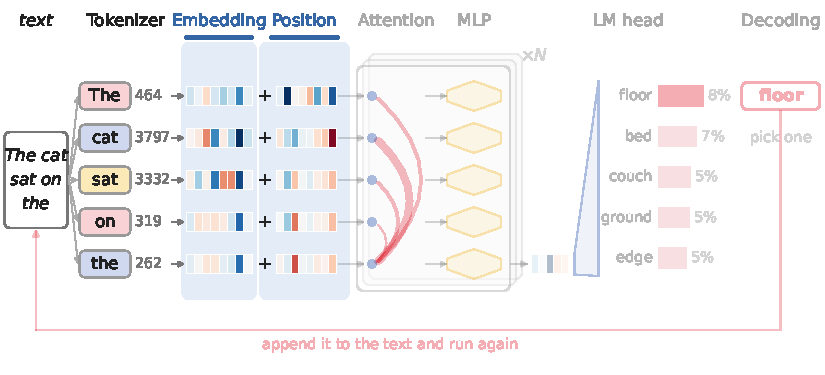
\includegraphics[width=\linewidth]{roadmap_embeddings_pass.pdf}\end{center}
  \vskip -2pt
  {\small Today: the next two boxes - an ID becomes a vector, and the vector learns where it sits.}
\end{frame}

\begin{frame}{Where we are: the life of a model}
  \begin{center}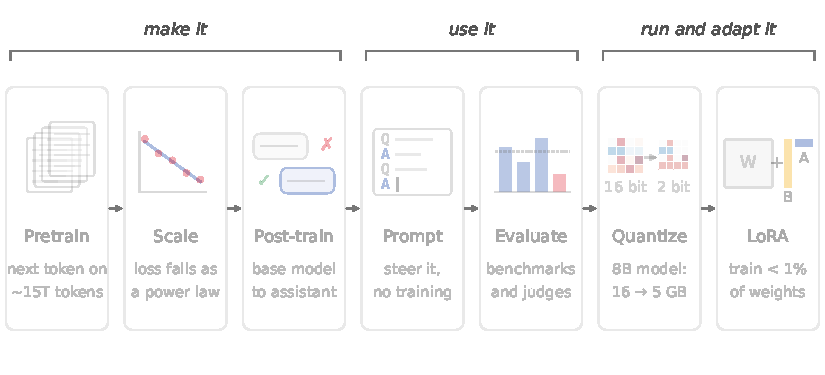
\includegraphics[width=\linewidth]{roadmap_embeddings_life.pdf}\end{center}
  \vskip -2pt
  {\small Later: where the weights come from, and what you do with them once you have them.}
\end{frame}

% ============================================================ COLD OPEN
\begin{frame}{Same words, opposite news}
  \begin{center}
    {\Large ``The dog bites the man''}\\[4pt]
    {\Large ``The man bites the dog''}
  \end{center}
  \vskip 2pt
  \textbf{Predict:} the model's first step looks every token up in a table and gets back a list of
  numbers. Are the two sentences still different after that step?
  \vfill
  \begin{center}
    
\includegraphics[width=3.0in]{emb_kargin.pdf}\\[-2pt]
    \src{\href{https://karginhaghordum.am/sketch/3bEwVKXicsQ/}{karginhaghordum.am/sketch/3bEwVKXicsQ}}
  \end{center}
\end{frame}

\begin{frame}{Same five numbers, same five vectors}
  \begin{center}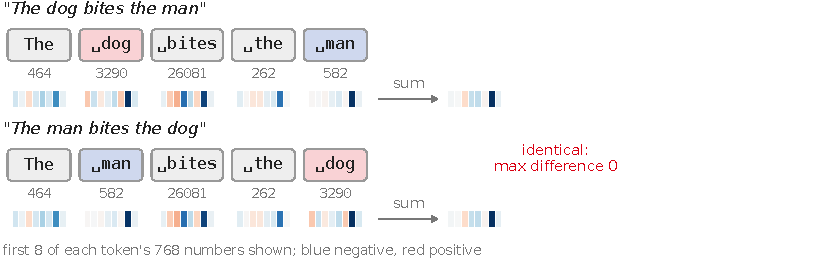
\includegraphics[width=\linewidth]{emb_coldopen_ids.pdf}\end{center}
  \vskip -4pt
  {\small The same five token IDs in a different order. Each ID fetches its row of the table, so
  both sentences arrive as the \textbf{same five vectors}. Add them up and the totals agree to
  the last bit.}
  \vskip 4pt
  \watchbox{Aside: without ``The'', ``dog bites man'' and ``man bites dog'' are not even the same
  tokens. The first word has no space before it, and ``dog'' is a different token from ``\,dog''
  (LLM-1).}
\end{frame}

\begin{frame}{Outline}
  \tableofcontents
\end{frame}

% ============================================================ 1. ID -> VECTOR
\section{An ID becomes a vector}
\sectiontransition{An ID becomes a vector}{3290 is a row number, not a quantity.}

\begin{frame}{An ID is a name, not a number}
  \begin{itemize}
    \item LLM-1 ended with integers: `` cat'' is \textbf{3797}, `` dog'' is \textbf{3290}.
    \item Is a cat 507 ``more'' than a dog? Is `` dog'' + 1 a puppy? The IDs were handed out by
      the order of BPE's merges. Their sizes mean nothing.
    \item L20 hit the same wall with one-hot vectors: every word equally far from every other,
      so ``cat'' is no closer to ``dog'' than to ``Tuesday''.
  \end{itemize}
  \vskip 10pt
  \keybox{What we want: one list of numbers per token, where tokens used in similar ways get
  similar numbers. And we want the model to \textbf{learn} those numbers, not us to choose them.}
\end{frame}

\begin{frame}{By hand: a one-hot vector times a matrix picks a row}
  \small
  A 4-token vocabulary (the, cat, sat, on), 3 numbers per token. The table $E$ has one row per
  token. ``cat'' is token 1, so its one-hot vector has a 1 in place 1:
  \[
    \underbrace{\begin{pmatrix} 0 & 1 & 0 & 0 \end{pmatrix}}_{\text{one-hot(cat)}}
    \underbrace{\begin{pmatrix}
      \phantom{-}0.2 & -0.1 & \phantom{-}0.5 \\
      \phantom{-}0.9 & \phantom{-}0.3 & -0.4 \\
      -0.6 & \phantom{-}0.8 & \phantom{-}0.1 \\
      \phantom{-}0.0 & -0.5 & \phantom{-}0.7
    \end{pmatrix}}_{E \text{ (4 tokens} \times \text{3 numbers)}}
    = 0 \cdot \text{row}_0 + 1 \cdot \text{row}_1 + 0 \cdot \text{row}_2 + 0 \cdot \text{row}_3
    = \begin{pmatrix} 0.9 & 0.3 & -0.4 \end{pmatrix}
  \]
  \vskip -2pt
  \begin{itemize}
    \item Every zero wipes out a row; the single 1 keeps row 1. So the ``embedding layer'' is a
      matrix multiplication that is really a \textbf{table lookup}: code just reads row 1.
    \item Training works the same way: the gradient reaches only the rows that were looked up.
      A token that never shows up in training never moves.
  \end{itemize}
\end{frame}

\begin{frame}{GPT-2's table}
  \begin{columns}[T]
    \begin{column}{0.40\textwidth}
      \small
      \begin{itemize}
        \item One row per token: \textbf{50,257} rows.
        \item 768 numbers per row.
        \item $50{,}257 \times 768 = 38{,}597{,}376$ numbers: \textbf{31.0\%} of GPT-2 small's
          124M parameters (LLM-1's vocabulary trade-off).
      \end{itemize}
    \end{column}
    \begin{column}{0.58\textwidth}
      \vskip -2pt
      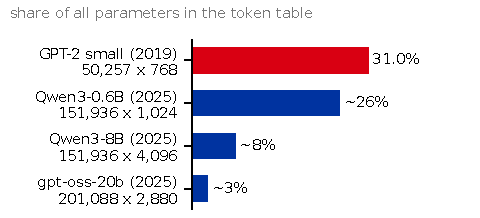
\includegraphics[width=\linewidth]{emb_table_sizes.pdf}
    \end{column}
  \end{columns}
  \vskip 8pt
  {\small Bigger models spend a smaller share on it: the table grows with the vocabulary and the
  width, the rest of the model grows much faster.}
  \vskip 2pt
  \src{Qwen3 and gpt-oss: vocabulary and width from their config.json, totals from their model
  cards (rounded there, hence ``\textasciitilde''), checked 4 Oct 2026.}
\end{frame}

\begin{frame}{Who fills the table?}
  \begin{itemize}
    \item At the start: small random numbers. ``cat'' and ``dog'' are as unrelated as any two
      rows.
    \item Then the table trains with the rest of the model, by backpropagation, on one task:
      predict the next token. Nobody ever tells it what a cat is.
    \item You have built one already: the ch11 name inventor was \textbf{an embedding table plus
      an MLP}. Its table had 40 rows (38 letters, plus the start and end symbols). Same idea,
      now with 50,257 rows.
  \end{itemize}
  \vskip 10pt
  \keybox{If two tokens keep appearing in the same places, the gradient keeps pushing their
  rows in the same direction. Similar use $\Rightarrow$ similar rows. Let us check whether that
  happened.}
\end{frame}

\begin{frame}{Predict first}
  \vskip 30pt
  \begin{center}
    {\Large\color{popblue}\textbf{Which rows of GPT-2's table sit closest to `` Monday''?}}
    \vskip 14pt
    {\small Closest = largest cosine similarity (the angle between two rows).}
    \vskip 24pt
    {\small\color{gray}Commit to an answer.}
  \end{center}
\end{frame}

\begin{frame}{What the table learned}
  \begin{center}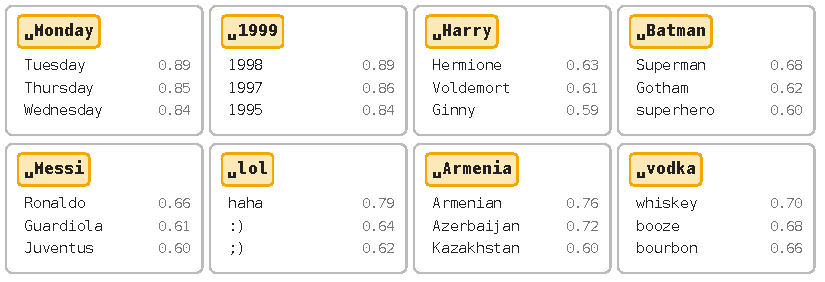
\includegraphics[width=\linewidth]{emb_neighbours.pdf}\end{center}
  \vskip -4pt
  {\small The three nearest rows of each word, with their cosine similarity. Days next to days,
  years next to years, Hermione next to Harry, Ronaldo next to Messi. Spelling variants of the
  word itself are skipped here (next slide).}
  \vskip 4pt
  \takebox{Nobody labelled a single token. All of this came from predicting the next one.}
\end{frame}

\begin{frame}{Neighbours share contexts, not meanings}
  \begin{center}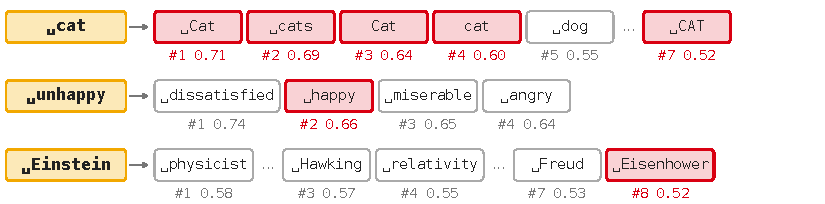
\includegraphics[width=\linewidth]{emb_neighbours_odd.pdf}\end{center}
  \vskip -4pt
  \small
  \begin{itemize}
    \item `` cat'': the nearest rows are the same word spelled differently. LLM-1's tokenizer
      gave them separate IDs; training pulled their rows back together.
    \item `` unhappy'': its second neighbour is its \textbf{opposite}. ``I was \underline{\ \ \ \ }
      with the result'' takes both. Opposites live in the same places.
    \item `` Einstein'': physicists, then at \#8 `` Eisenhower'': another famous 20th-century
      name, with similar letters. Not physics.
  \end{itemize}
  \vskip 2pt
  \watchbox{A row records how a token is \textbf{used}. Usually that tracks meaning. Not always.}
\end{frame}

\begin{frame}{The glitch tokens found each other}
  \begin{center}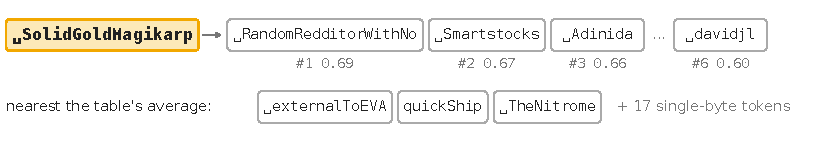
\includegraphics[width=\linewidth]{emb_glitch.pdf}\end{center}
  \vskip -2pt
  \small
  \begin{itemize}
    \item LLM-1's glitch token's nearest rows are \textbf{other glitch tokens}: Reddit user names
      and scraped-page leftovers.
    \item The 20 rows closest to the table's average row: these three, plus 17 single-byte
      tokens.
    \item Why: these tokens were in the tokenizer's training text and almost never in the
      model's. Their rows got almost no gradient (the lookup slide), so they stayed close to
      where they started, close to each other.
  \end{itemize}
  \vskip 2pt
  \src{Land \& Bartolo (2024), ``Fishing for Magikarp'', EMNLP: thousands of such under-trained
  tokens in today's open models, found from the weights alone.}
\end{frame}

\begin{frame}{Directions carry meaning (mostly)}
  \small
  Take row $b$, subtract row $a$, add row $c$, and ask which row is nearest:
  \vskip 4pt
  \begin{center}
  \begin{tabular}{lll}
    \textbf{query} & \textbf{nearest row} & \textbf{cosine} \\
    \hline
    king $-$ man $+$ woman & \textcolor{paramgreen}{\textbf{queen}} & 0.69 \\
    actor $-$ man $+$ woman & \textcolor{paramgreen}{\textbf{actress}} & 0.82 \\
    cats $-$ cat $+$ mouse & \textcolor{paramgreen}{\textbf{mice}} (an irregular plural) & 0.70 \\
    German $-$ Germany $+$ Armenia & \textcolor{paramgreen}{\textbf{Armenian}} & 0.79 \\
    better $-$ good $+$ bad & \textcolor{paramgreen}{\textbf{worse}} & 0.63 \\
    \hline
    Paris $-$ France $+$ Italy & \textcolor{armred}{``Paris'' (no space), Milan; Rome only 5th} & 0.62 \\
    walked $-$ walk $+$ swim & \textcolor{armred}{swimming, not swam} & 0.61 \\
  \end{tabular}
  \end{center}
  \vskip 4pt
  \watchbox{Fine print: the three input words are removed from the answers, as everyone does
  (Mikolov et al., 2013). Without that rule, 3 of the 5 green rows answer with one of their own
  inputs: king $-$ man $+$ woman is nearest to \textbf{king} (Nissim et al., 2020, make this
  point). So: a real tendency of the table, not a law.}
\end{frame}

\begin{frame}{One row per token, whatever the sentence}
  \begin{itemize}
    \item ``We sat on the river \textbf{bank}'' and ``I opened a \textbf{bank} account'': both
      ``\,bank''s are token 3331, so both get \textbf{the same row}.
    \item The table cannot see the sentence. It answers ``which token is this?'', never ``what
      does it mean here?''.
    \item Telling the two banks apart is the job of the next layers, which mix each vector with
      its neighbours (L24).
  \end{itemize}
  \vskip 10pt
  \keybox{The table gives each token a \textbf{starting point}. The vectors that come out of the
  last layer are different for every occurrence of a token; the ones that go in are not.}
\end{frame}

\begin{frame}{The same table, used twice}
  \begin{itemize}
    \item At the very end, the model must turn its last vector back into a token: score the
      vector against every token, pick from the scores (L26, then LLM-3).
    \item GPT-2 scores it against \textbf{the same 50,257 rows}: one table for reading tokens in
      and for writing them out. This is called \textbf{tying} the input and output embeddings.
    \item Small models tie, big ones usually keep two tables. Tied: Qwen3-0.6B, Gemma 4 E2B. Not
      tied: Qwen3-8B, gpt-oss-20b, DeepSeek-V3.
  \end{itemize}
  \vskip 10pt
  \takebox{Sharing works because both jobs want the same thing: tokens used alike get vectors
  alike. Why the split: in a small model the table is a quarter or more of all parameters (the
  GPT-2 slide), so sharing it saves a lot. In a big one it is a few percent.}
  \vskip 4pt
  \src{\texttt{tie\_word\_embeddings} in each model's config.json, checked 4 Oct 2026.}
\end{frame}

% ============================================================ 2. WHERE IS THE ORDER
\section{Where is the order?}
\sectiontransition{Where is the order?}{A table lookup has no idea where the token sat.}

\begin{frame}{Back to the dog}
  \begin{itemize}
    \item `` dog'' is the 2nd token of ``The dog bites the man'' and the 5th of ``The man bites
      the dog''. The table hands back the same row both times.
    \item So after the lookup, each sentence is just \textbf{five vectors}, and they are the same
      five. The model has received a \textbf{set}: which vectors, but not in what order.
    \item ``Dog bites man'' is not news. ``Man bites dog'' is. The difference is entirely in the
      order.
  \end{itemize}
  \vskip 10pt
  \keybox{Writing the vectors in a list on the slide gives them an order. The question is
  whether anything \textbf{inside the model} can tell which one was first.}
\end{frame}

\begin{frame}{Why the next layer cannot recover it}
  \small
  A preview of L24. The next layer updates each vector like this:
  \begin{enumerate}
    \item compare it with every other vector: a \textbf{dot product} of their numbers;
    \item turn those scores into weights;
    \item add the vectors up with those weights.
  \end{enumerate}
  \vskip 4pt
  Each step uses only \textbf{what is in} the vectors. None of them reads a slot number, and a
  weighted sum gives the same total whatever order you add in. Next slide: by hand. The
  attention lecture proves it in general: shuffle the inputs and every output comes back
  unchanged, just shuffled.
  \vskip 8pt
  \keybox{An RNN never had this problem: it read tokens one at a time, so order was built into
  the computation (L20). Attention reads all tokens at once - that is why it is fast - and the
  price is that order is gone.}
\end{frame}

\begin{frame}{By hand: shuffle the sentence, and nothing changes}
  \small
  Toy vectors with 2 numbers: dog $= (1, 0)$, bites $= (1, 1)$, man $= (0, 1)$. The next layer,
  simplified (L24 adds learned matrices), updates ``dog'':
  \vskip 2pt
  \begin{center}
  \begin{tabular}{l|lcc|lcc}
    & \multicolumn{3}{c|}{\textbf{dog bites man}} & \multicolumn{3}{c}{\textbf{man bites dog}} \\
    slot & vector & score & weight & vector & score & weight \\
    \hline
    0 & dog $(1, 0)$ & 1 & 0.42 & man $(0, 1)$ & 0 & 0.16 \\
    1 & bites $(1, 1)$ & 1 & 0.42 & bites $(1, 1)$ & 1 & 0.42 \\
    2 & man $(0, 1)$ & 0 & 0.16 & dog $(1, 0)$ & 1 & 0.42 \\
  \end{tabular}
  \end{center}
  \vskip 2pt
  \begin{enumerate}
    \item Score: the dot product with dog's vector. dog $\cdot$ bites $= 1 \cdot 1 + 0 \cdot 1 = 1$.
    \item Weight: softmax of the scores, as in multiclass classification: $e^1, e^1, e^0$
      divided by their sum gives $0.42, 0.42, 0.16$.
    \item Output: $0.42 \cdot (1, 0) + 0.42 \cdot (1, 1) + 0.16 \cdot (0, 1) =
      \mathbf{(0.84,\; 0.58)}$ - in \textbf{both} sentences.
  \end{enumerate}
  \vskip 2pt
  \keybox{Each weight travels with its vector, not with its slot. Shuffling the sentence only
  shuffles the rows of this table.}
\end{frame}

\begin{frame}{The fix: write the slot into the vector}
  \small
  Give every \textbf{slot} its own vector too, and add it to the token's row:
  \[
    \text{input}_i \;=\; \underbrace{E[\text{token}_i]}_{\text{which token}}
      \;+\; \underbrace{P[i]}_{\text{which slot}}
  \]
  \begin{center}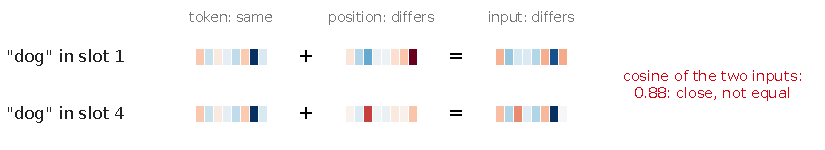
\includegraphics[width=\linewidth]{emb_add_position.pdf}\end{center}
  \vskip -4pt
  Now ``dog in slot 1'' and ``dog in slot 4'' are different inputs, and anything that compares
  vectors can tell them apart. Real GPT-2 rows above: the first 8 of 768 numbers.
\end{frame}

\begin{frame}{By hand: add positions, and dog's output changes}
  \small
  Same toy, plus a vector per slot: slot 0 $= (0.5, 0)$, slot 1 $= (0, 0)$, slot 2 $= (0, 0.5)$.
  Add them, then run the same three steps for ``dog'':
  \vskip 2pt
  \begin{center}
  \begin{tabular}{l|lcc|lcc}
    & \multicolumn{3}{c|}{\textbf{dog bites man}} & \multicolumn{3}{c}{\textbf{man bites dog}} \\
    slot & input & score & weight & input & score & weight \\
    \hline
    0 & dog $(1.5, 0)$ & 2.25 & 0.63 & man $(0.5, 1)$ & 1.00 & 0.25 \\
    1 & bites $(1, 1)$ & 1.50 & 0.30 & bites $(1, 1)$ & 1.50 & 0.42 \\
    2 & man $(0, 1.5)$ & 0 & 0.07 & dog $(1, 0.5)$ & 1.25 & 0.33 \\
    \hline
    & \multicolumn{3}{l|}{dog's output: $\mathbf{(1.25,\; 0.40)}$} &
      \multicolumn{3}{l}{dog's output: $\mathbf{(0.87,\; 0.84)}$} \\
  \end{tabular}
  \end{center}
  \vskip 4pt
  ``dog'' is now a different vector in each sentence ($(1.5, 0)$ in slot 0, $(1, 0.5)$ in slot
  2), so every score changes, so the weights and the output change.
  \vskip 6pt
  \takebox{Same words, different outputs: the layer can now tell who bit whom. Yet the three
  inputs still add up to $(2.5, 2.5)$ in both sentences. That is the trap on the next slide.}
\end{frame}

\begin{frame}{Trap: adding positions does not fix a sum}
  \vskip 4pt
  Take the cold open again, with position vectors added this time, and add up the five inputs:
  \[
    \sum_i \big(E[\text{token}_i] + P[i]\big) \;=\; \sum_i E[\text{token}_i] \;+\; \sum_i P[i]
  \]
  Both sentences have the same tokens and the same five slots, so both sums are the same. We
  measured it on GPT-2: the two totals still agree to the last bit. The toy said the same:
  $(2.5, 2.5)$ twice.
  \vskip 10pt
  \trapbox{Positions do not change the \textbf{total}; they change \textbf{each vector}. That is
  enough, because the next layer compares vectors pair by pair before it adds anything up (last
  slide: dog's output moved from $(1.25, 0.40)$ to $(0.87, 0.84)$). A model that only summed or
  averaged its inputs would stay blind to order.}
\end{frame}

% ============================================================ 3. LEARNED POSITIONS
\section{Option 1: learn the positions}
\sectiontransition{Option 1: learn the positions}{Another table, one row per slot.}

\begin{frame}{GPT-2's position table}
  \begin{itemize}
    \item A second table, $P$: one row per slot, 768 numbers per row, trained by
      backpropagation exactly like the token table.
    \item It has \textbf{1,024} rows: 786,432 numbers, 0.63\% of GPT-2. Cheap.
    \item Slot 1,025 has no row. GPT-2 cannot read a 1,025th token at all: the limit is built
      into the shape of a matrix. This limit is the model's \textbf{context length}: the most
      tokens it can read at once.
    \item BERT (2018) did the same with 512 rows. Longer documents had to be cut into pieces.
  \end{itemize}
  \vskip 10pt
  \keybox{Nobody told GPT-2 that slot 7 comes between slots 6 and 8. To the training
  procedure they are 1,024 unrelated rows.}
\end{frame}

\begin{frame}{Predict first}
  \vskip 30pt
  \begin{center}
    {\Large\color{popblue}\textbf{After training, what do those 1,024 rows look like?}}
    \vskip 14pt
    {\small Random noise? Something smooth? Something else?}
    \vskip 24pt
    {\small\color{gray}Commit to an answer.}
  \end{center}
\end{frame}

\begin{frame}{It learned waves on its own}
  \begin{center}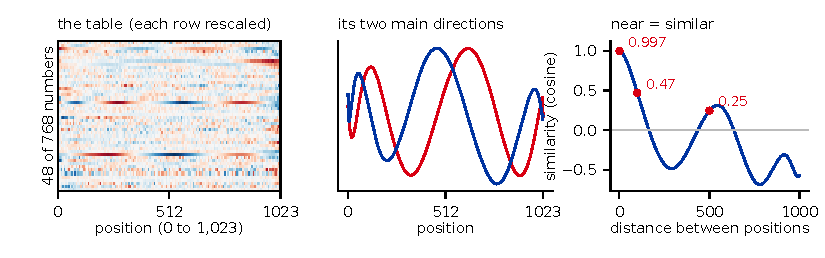
\includegraphics[width=\linewidth]{emb_gpt2_positions.pdf}\end{center}
  \vskip -4pt
  \small
  \begin{itemize}
    \item Right: average cosine between two slots' rows, by distance. Neighbours \textbf{0.997},
      100 apart 0.47, then it oscillates.
    \item Middle: PCA (ch10) on the 1,024 rows. 3 components hold 90\% of the variance; the two
      biggest, plotted over the slots, are slow waves.
  \end{itemize}
  \vskip 2pt
  \takebox{Order was learned from scratch, smooth and wave-like. Remember that for option 2.}
\end{frame}

\begin{frame}{Learned positions: the bill}
  \begin{itemize}
    \item \textbf{A hard length limit.} The table has as many rows as the longest training text,
      and no row exists beyond it.
    \item \textbf{Nothing carries over.} Slot 2,000 cannot be guessed from slots 1 to 1,024: a
      new row needs training data at that length.
    \item \textbf{Absolute, not relative.} ``Three slots back'' has to be learned separately for
      slot 10, slot 500 and slot 1,000. Nothing in the setup says they are the same idea.
  \end{itemize}
  \vskip 10pt
  \keybox{The waves on the last slide suggest a cheaper route: if smooth waves are what the
  model wants, write them down instead of learning them.}
\end{frame}

% ============================================================ 4. SINUSOIDS
\section{Option 2: write the positions down}
\sectiontransition{Option 2: write the positions down}{No training, and a value for every slot.}

\begin{frame}{A clock with many hands}
  \small
  The original Transformer (Vaswani et al., 2017) fixes $P$ with a formula. For slot $pos$ and
  dimension pair $i$ (of $d$ dimensions):
  \[
    P_{pos,\,2i} = \sin\!\left(\frac{pos}{10000^{2i/d}}\right) \qquad
    P_{pos,\,2i+1} = \cos\!\left(\frac{pos}{10000^{2i/d}}\right)
  \]
  \vskip -4pt
  \begin{center}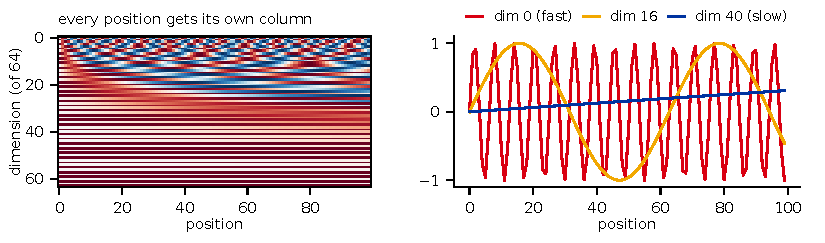
\includegraphics[width=\linewidth]{emb_sinusoid_heatmap.pdf}\end{center}
  \vskip -6pt
  Each pair of dimensions is a clock hand turning at its own speed. Fast hands tell neighbours
  apart; slow hands tell far-apart slots apart. Together they give every slot a unique reading.
\end{frame}

\begin{frame}{Similarity depends on the gap only}
  \begin{columns}[T]
    \begin{column}{0.60\textwidth}
      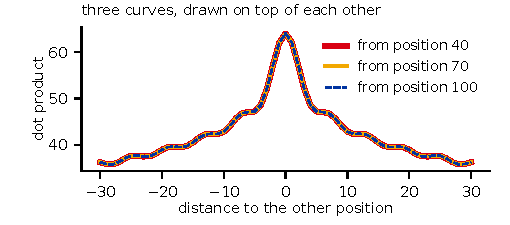
\includegraphics[width=\linewidth]{emb_sinusoid_gap.pdf}
    \end{column}
    \begin{column}{0.38\textwidth}
      \small
      The dot product of two slots' vectors, starting from slots 40, 70 and 100: the three curves
      are \textbf{identical} (largest difference below $10^{-9}$). Only the distance matters,
      not where you are.
    \end{column}
  \end{columns}
  \vskip 6pt
  \keybox{So ``three slots back'' looks the same at slot 10 and at slot 1,000: learn it once.}
  \vskip 4pt
  \trapbox{The formula has a value for every slot, so it seems to promise texts longer than any
  seen in training. In practice it does not deliver: trained on 512 or 1,024 tokens, such
  models get worse soon after the training length (Press et al., 2022). The model never learned
  to use the unseen readings.}
\end{frame}

\begin{frame}{Why only the gap: one identity}
  \small
  Take one pair of dimensions, with speed $\omega$, at slots $a$ and $b$. Its share of the dot
  product $P_a \cdot P_b$ is
  \[
    \sin(\omega a)\sin(\omega b) + \cos(\omega a)\cos(\omega b) \;=\; \cos\big(\omega (a - b)\big)
  \]
  (the cosine-of-a-difference identity). Add up all $d/2$ pairs:
  \[
    P_a \cdot P_b \;=\; \sum_{i} \cos\big(\omega_i\,(a - b)\big),
    \qquad \omega_i = \frac{1}{10000^{2i/d}}
  \]
  \vskip -2pt
  \begin{itemize}
    \item Only $a - b$ is left: the address cancels. That is why the three curves were one.
    \item At gap 0 every term is $\cos 0 = 1$, so the dot product peaks at $d/2$: 64 in the plot,
      where $d = 128$.
    \item Further apart, the pairs turn at different speeds and drift out of step; their terms
      partly cancel. Those are the wobbles.
  \end{itemize}
  \vskip 4pt
  \keybox{Hold on to $\cos(\omega(a - b))$: RoPE (option 3) is built on exactly this identity.}
\end{frame}

\begin{frame}{Predict first}
  \vskip 26pt
  \begin{center}
    {\Large\color{popblue}\textbf{Every model here \emph{adds} the position vector\\ to the token
    vector. Why not put them side by side?}}
    \vskip 14pt
    {\small Adding mixes two kinds of information into the same 768 numbers. Surely that blurs
    the token?}
    \vskip 24pt
    {\small\color{gray}Commit to an answer.}
  \end{center}
\end{frame}

\begin{frame}{By hand: adding can be concatenation in disguise}
  \small
  A toy with 4 numbers per vector. Tokens use the first two, slots the last two:
  \[
    \text{dog} = (3, 1, 0, 0) \quad \text{cat} = (1, 3, 0, 0) \qquad
    \text{slot 1} = (0, 0, 1, 0) \quad \text{slot 4} = (0, 0, 0, 1)
  \]
  \[
    \text{dog in slot 4} = (3, 1, 0, 0) + (0, 0, 0, 1) = (3, 1, 0, 1)
  \]
  \begin{itemize}
    \item The first two numbers still say ``dog'': the dot product with dog is
      $3 \cdot 3 + 1 \cdot 1 = 10$, with cat only $3 \cdot 1 + 1 \cdot 3 = 6$.
    \item The last two numbers say ``slot 4''. Nothing was blurred.
    \item Putting them side by side, $(3, 1 \,|\, 0, 1)$, is the same thing, except that every
      later layer must be wider to accept the longer vector.
  \end{itemize}
  \vskip 4pt
  \keybox{If tokens and slots live in \textbf{different directions}, adding them loses nothing.
  The question is whether a real model keeps them apart.}
\end{frame}

\begin{frame}{Measured: 768 dimensions leave room}
  \begin{columns}[T]
    \begin{column}{0.62\textwidth}
      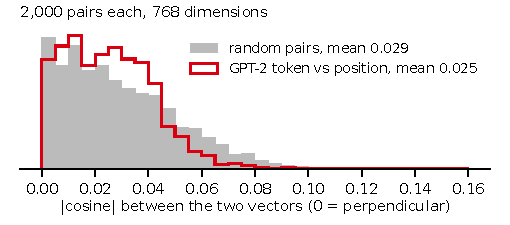
\includegraphics[width=\linewidth]{emb_add_vs_concat.pdf}
    \end{column}
    \begin{column}{0.36\textwidth}
      \small
      GPT-2's token rows and position rows are \textbf{almost perpendicular}: average
      $|\cos|$ 0.025, even closer than random pairs (0.029).
    \end{column}
  \end{columns}
  \vskip 6pt
  \small
  \begin{itemize}
    \item Add a random position to a random token, then ask which token row is nearest: the right
      one, \textbf{1,998 times out of 2,000}.
    \item The 2 misses: a stray byte and `` RandomRedditor'', a glitch token. The barely-trained
      rows again.
  \end{itemize}
  \vskip 2pt
  \takebox{In high dimensions, almost every pair of directions is nearly perpendicular. Adding is
  cheap and keeps both messages readable.}
\end{frame}

% ============================================================ 5. ROPE
\section{Option 3: rotate, do not add}
\sectiontransition{Option 3: rotate, do not add}{What a comparison needs is the gap, not the
address.}

\begin{frame}{What we actually want}
  \begin{itemize}
    \item The next layer compares pairs of tokens (L24). From each token's vector it makes two
      new ones: a \textbf{query} (``what am I looking for?'') and a \textbf{key} (``what do I
      offer?''). The score of a pair is query $\cdot$ key, the dot product from the toy.
    \item For that score, what matters is ``these two are 3 apart'', not ``one is in slot 41 and
      the other in slot 44''.
    \item Adding a position vector bakes in the \textbf{address}. Sinusoids make the gap
      recoverable, but the model still has to learn to dig it out of the sum.
    \item Better: build the comparison so that \textbf{only the gap can affect it}.
  \end{itemize}
  \vskip 10pt
  \keybox{Rotary Position Embedding (RoPE; Su et al., 2021): instead of adding a position vector,
  \textbf{rotate} the vector by an angle proportional to its slot.}
\end{frame}

\begin{frame}{Each pair of numbers is a clock hand}
  \begin{center}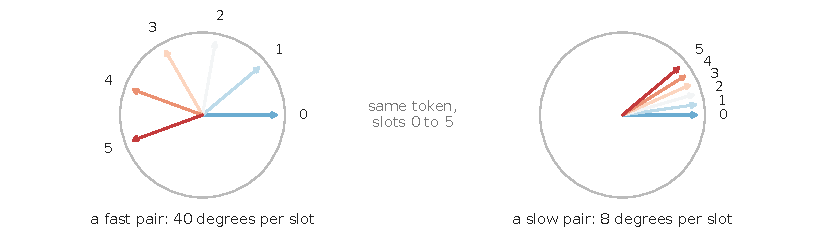
\includegraphics[width=\linewidth]{emb_rope_clock.pdf}\end{center}
  \vskip -4pt
  \small
  \begin{itemize}
    \item Split the vector into pairs of numbers. Treat each pair as an arrow in 2-D.
    \item In slot $m$, turn every arrow by $m \times \theta$. Pair $i$ has its own speed
      $\theta_i = 1 / 10000^{2i/d}$, the sinusoids' speeds: with 128 numbers per head, 64 pairs,
      from 1 radian per slot down to 0.000115.
    \item The arrow's length never changes: only its direction carries the slot.
  \end{itemize}
\end{frame}

\begin{frame}{Why only the gap survives}
  \begin{center}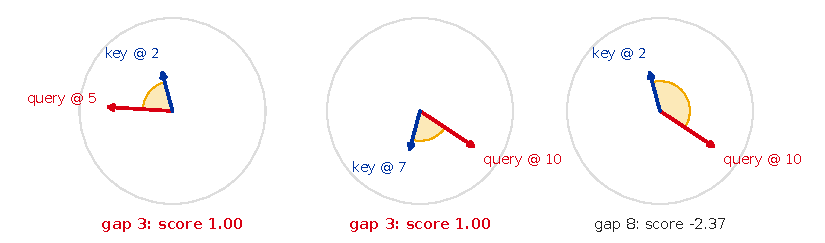
\includegraphics[width=\linewidth]{emb_rope_2d.pdf}\end{center}
  \vskip -6pt
  \small
  A dot product depends on two lengths and the angle between the arrows:
  $\mathbf{q} \cdot \mathbf{k} = |\mathbf{q}|\,|\mathbf{k}| \cos(\text{angle between})$.
  Turn the query by $m\theta$ and the key by $n\theta$: the angle between them changes by
  $(m - n)\,\theta$. The lengths do not change at all. So the score depends on the content and
  the \textbf{gap} $m - n$ only.
\end{frame}

\begin{frame}{By hand: same gap, same score}
  \small
  $\mathbf{q} = (2, 1)$, $\mathbf{k} = (1, 1)$, $\theta = 30^\circ$ per slot. Unrotated,
  $\mathbf{q} \cdot \mathbf{k} = 2 + 1 = 3$. Turning $(x, y)$ by an angle $\varphi$ gives
  $(x\cos\varphi - y\sin\varphi,\; x\sin\varphi + y\cos\varphi)$.
  \vskip 4pt
  \begin{center}
  \begin{tabular}{llll}
    \textbf{slots} & \textbf{query turned by} & \textbf{key turned by} & \textbf{score} \\
    \hline
    $q$ in 5, $k$ in 2 & $150^\circ$: $(-2.23,\; 0.13)$ & $60^\circ$: $(-0.37,\; 1.37)$ &
      $0.82 + 0.18 = \mathbf{1.00}$ \\
    $q$ in 10, $k$ in 7 & $300^\circ$: $(1.87,\; -1.23)$ & $210^\circ$: $(-0.37,\; -1.37)$ &
      $-0.68 + 1.68 = \mathbf{1.00}$ \\
    $q$ in 10, $k$ in 2 & $300^\circ$: $(1.87,\; -1.23)$ & $60^\circ$: $(-0.37,\; 1.37)$ &
      $-2.37$ \\
  \end{tabular}
  \end{center}
  \vskip 6pt
  Gap 3 gives 1.00 at slots 5/2 and at 10/7. Gap 8 gives something else. Check one row
  yourself: $\cos 150^\circ = -0.866$, $\sin 150^\circ = 0.5$, so the query becomes
  $(2 \cdot (-0.866) - 1 \cdot 0.5,\; 2 \cdot 0.5 + 1 \cdot (-0.866)) = (-2.23,\; 0.13)$.
  \vskip 6pt
  \takebox{The model never sees the slot numbers 5, 2, 10 or 7. It only ever feels the gap.}
\end{frame}

\begin{frame}{Where the rotation happens}
  \begin{itemize}
    \item Not at the input. The token vector goes in with \textbf{no} position added.
    \item The rotation is applied inside every attention layer, to the query and the key of each
      token, right before their dot product.
    \item So position enters each layer's comparison directly, instead of being added once at
      the bottom and carried through.
  \end{itemize}
  \vskip 10pt
  \keybox{On the map, the Position box stays where it is: it is still ``tell each vector where it
  sits''. With RoPE it does so inside the attention box, at every layer.}
\end{frame}

\begin{frame}{Who uses it}
  \begin{itemize}
    \item RoFormer (2021) reported modest gains. Adoption was anything but modest: GPT-J and
      GPT-NeoX, PaLM, then LLaMA (2023), and after LLaMA nearly every open model.
    \item Every 2024-2026 model in the table at the end of today uses RoPE in some form.
    \item Two reasons it won: the score depends only on the gap, and it adds no parameters at
      all - a rotation has nothing to learn.
  \end{itemize}
  \vskip 10pt
  \watchbox{One thing RoPE does not fix by itself: texts longer than the training ones. That is
  the last section.}
\end{frame}

\begin{frame}{Three options, side by side}
  \footnotesize
  \begin{center}
  \begin{tabular}{>{\raggedright\arraybackslash}p{2.2cm}>{\raggedright\arraybackslash}p{3.3cm}%
                  >{\raggedright\arraybackslash}p{3.3cm}>{\raggedright\arraybackslash}p{3.3cm}}
    & \textbf{learned table} (GPT-2) & \textbf{sinusoids} (2017) & \textbf{RoPE} (2021) \\
    \hline
    what it does & adds a trained row per slot & adds a fixed wave pattern & rotates query and key
      inside attention \\[2pt]
    parameters & one row per slot (786,432 numbers in GPT-2) & none & none \\[2pt]
    ``3 slots apart'' & learned separately at every slot & the same pattern everywhere; the model
      must dig it out & the score sees only the gap \\[2pt]
    past the training length & impossible: no row exists & allowed, but quality drops & allowed,
      but quality drops; can be stretched (next section) \\
  \end{tabular}
  \end{center}
  \vskip 8pt
  \keybox{Each option fixes something in the column before it: sinusoids drop the trained rows
  and make the gap the same everywhere; RoPE makes the gap the \textbf{only} thing a comparison
  can see. None of them, by itself, makes a model good at lengths it never trained on.}
\end{frame}

% ============================================================ 6. LONGER AND LONGER
\section{Longer and longer}
\sectiontransition{Longer and longer}{GPT-2 stopped at 1,024 tokens. Models now read hundreds of
thousands.}

\begin{frame}{Why RoPE breaks past its training length}
  \begin{center}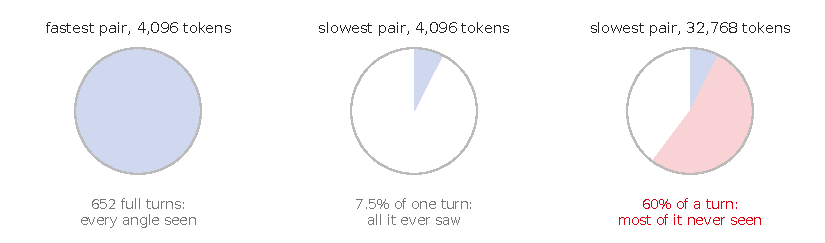
\includegraphics[width=\linewidth]{emb_rope_unseen.pdf}\end{center}
  \vskip -6pt
  \small
  A model trained on 4,096 tokens, RoPE base 10,000, 128 numbers per head (Llama 2's
  settings). The fastest hand spins about 650 times during one training text: it has seen every
  angle. The slowest turns 0.000115 radians per slot: $4{,}096 \times 0.000115 = 0.47$ radians,
  only \textbf{7.5\%} of a circle. Feed it 32,768 tokens and that hand reaches 60\%: angles the
  model never saw, so the scores there are a guess.
  \vskip 2pt
  \src{Press et al. (2022) measured it: RoPE models hold up for 100-200 tokens past their training
  length, then get worse. Sinusoids fail sooner.}
\end{frame}

\begin{frame}{Stretch the clock}
  \begin{itemize}
    \item \textbf{Position interpolation} (Chen et al., 2023): divide every slot number by 8.
      Slot 32,000 is read as 4,000, an angle the model knows. But neighbours now differ by only
      1/8 of a step: harder to tell apart.
    \item \textbf{YaRN} (Yet another RoPE extensioN; Peng et al., 2024): stretch only the
      \textbf{slow} hands, the ones that never completed a turn. Leave the fast hands alone; they
      have seen every angle anyway.
    \item Then a short extra training run on long documents, so the model gets used to it.
  \end{itemize}
  \vskip 8pt
  \keybox{In 2025 configs: Qwen3-8B, native length 32,768 tokens, reaches 131,072 with YaRN.
  gpt-oss-20b was stretched from 4,096 to 131,072.}
  \vskip 2pt
  \src{Qwen3-8B model card; gpt-oss-20b config.json (\texttt{rope\_scaling}), checked 4 Oct
  2026.}
\end{frame}

\begin{frame}{Two other answers: a distance penalty, or no position at all}
  \begin{itemize}
    \item \textbf{Attention with Linear Biases} (ALiBi; Press et al., 2022): no position vectors
      at all. Each comparison score just gets a penalty that grows with the distance, so near
      tokens win unless a far one is much more relevant. BLOOM (2022) used it.
    \item \textbf{No Positional Encoding} (NoPE): nothing. A model that may only look back at
      earlier tokens (decoder models, L26) still works out positions on its own (Haviv et al.,
      2022): token 3 sees 3 tokens, token 300 sees 300, and that count gives its position away.
    \item Llama 4 (2025) mixes RoPE and NoPE: some layers rotate, some have no position at
      all. Meta reports up to 10 million tokens of context for Llama 4 Scout.
  \end{itemize}
  \vskip 6pt
  \takebox{Position is still an open design question. The 2017 answer did not last, and the
  2021 answer keeps being patched.}
\end{frame}

\begin{frame}{What models use, 2017-2026}
  \footnotesize
  \begin{center}
  \begin{tabular}{lll}
    \textbf{model} & \textbf{position} & \textbf{context (tokens)} \\
    \hline
    Transformer (2017) & sinusoids & - \\
    BERT (2018) & learned table & 512 \\
    GPT-2 (2019) & learned table & 1,024 \\
    T5 (2019) & a learned bias per distance & 512 in training \\
    BLOOM (2022) & ALiBi & 2,048 \\
    DeepSeek-V3 (2024) & RoPE + YaRN (from 4,096) & 163,840 \\
    Qwen3-8B (2025) & RoPE, base 1,000,000 & 32,768; 131,072 with YaRN \\
    gpt-oss-20b (2025) & RoPE + YaRN (from 4,096) & 131,072 \\
    Llama 4 Scout (2025) & RoPE layers + NoPE layers & 10,000,000 \\
    Gemma 4 E2B (2026) & RoPE, two bases: 10,000 and 1,000,000 & 131,072 \\
  \end{tabular}
  \end{center}
  \vskip 4pt
  {\small Gemma's two bases: layers that only look at nearby tokens use the faster clock
  (10,000), layers that see the whole text the slower one.}
  \vskip 2pt
  \src{config.json and model cards on Hugging Face, Meta's Llama 4 announcement; checked 4 Oct
  2026.}
\end{frame}

% ============================================================ RECAP
\section*{Recap}

\begin{frame}{Recap}
  \begin{itemize}
    \item An ID picks a \textbf{row of a learned table} (one-hot times a matrix). The rows
      learn how tokens are used: days near days, opposites near each other, glitch tokens in a
      pile.
    \item A lookup ignores order: both dog sentences arrive as the same five vectors.
    \item So each vector also gets its \textbf{slot}: a learned row (GPT-2, hard limit 1,024), a
      formula (sinusoids), or a rotation inside every attention layer (RoPE: only the gap
      counts).
    \item Adding works because in 768 dimensions token and position directions barely overlap.
    \item Longer texts: stretch the slow clock hands (YaRN), or penalise distance (ALiBi), or
      drop position in some layers (NoPE).
  \end{itemize}
\end{frame}

\begin{frame}{Next on the map}
  \begin{center}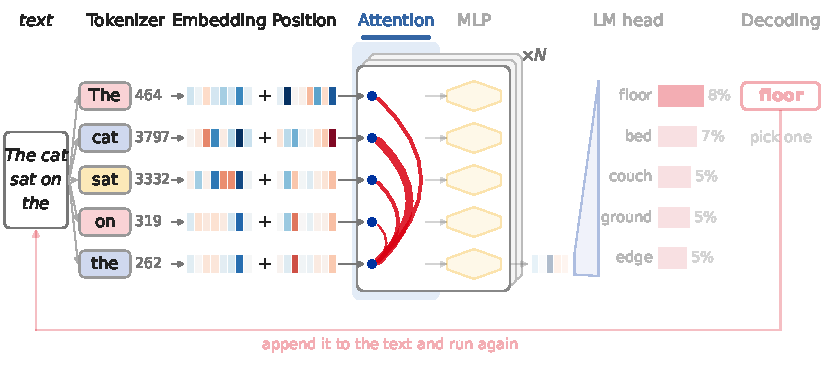
\includegraphics[width=\linewidth]{roadmap_attention_pass.pdf}\end{center}
  \vskip -2pt
  {\small Next (L24): the vectors start talking to each other.}
\end{frame}

\begin{frame}{Sources \& further reading}
  \footnotesize
  \begin{itemize}
    \item Vaswani et al. (2017), ``Attention Is All You Need'', NeurIPS (sinusoids).
    \item Su et al. (2021), ``RoFormer: Enhanced Transformer with Rotary Position Embedding'',
      arXiv; Neurocomputing (2024).
    \item Press, Smith \& Lewis (2022), ``Train Short, Test Long: Attention with Linear Biases
      Enables Input Length Extrapolation'', ICLR.
    \item Haviv et al. (2022), ``Transformer Language Models without Positional Encodings Still
      Learn Positional Information'', Findings of EMNLP.
    \item Chen et al. (2023), ``Extending Context Window of Large Language Models via Positional
      Interpolation'', arXiv; Peng et al. (2024), ``YaRN'', ICLR.
    \item Mikolov, Yih \& Zweig (2013), ``Linguistic Regularities in Continuous Space Word
      Representations'', NAACL; Nissim, van Noord \& van der Goot (2020), ``Fair is Better than
      Sensational'', Computational Linguistics.
    \item Land \& Bartolo (2024), ``Fishing for Magikarp'', EMNLP. Meta (April 2025), ``The Llama 4
      herd''.
  \end{itemize}
  \vskip 2pt
  \src{Every GPT-2 number: \texttt{py\_src/embeddings\_position\_figs.py} (GPT-2's weights read
  with safetensors, IDs from tiktoken), raw results in
  \texttt{results/embeddings\_position\_figs.json}.}
\end{frame}

\end{document}

% ============================================================================
% Provenance:
%   Deck: LLM-2 Embeddings and position (14_llms), session 2 of the LLM chapter (DECISIONS #68).
%   Built 2026-10-04 from LLM2_embeddings_position_OUTLINE.md (instructor interview 2026-10-04:
%   "id like positional encodings to be there, were going left to right") and
%   LLM_CHAPTER_PLAN.md, section 5 (LLM-2).
%   Moved here, not copied: L24's embedding primer ("Recall: a token is a vector", "Directions
%   carry meaning", "Embeddings soak up context") and L25's Position section (5 frames).
%   L24 and L25 were not edited (instructor: reference material until their rework). Ported and
%   adapted: sources/llm_training/16_rope (RoPE paper deck: the clock-hand intuition, "what we
%   actually want", by hand same gap same score, adoption), sources/dl4nlp/02_transformers.tex
%   (position frames), sources/dl4nlp/16_long_context_attention.tex ("Positional encoding for
%   length", "Context window extension").
%   Interview decisions: cold open dog bites man, with the instructor's Kargin Haghordum line
%   (ուրա պարավը, բերեք ատամը քաշեմ) and link; measurements = GPT-2's learned positions and
%   nearest neighbours of more interesting words; long-context tail short, intuition only; by-hand
%   frames = lookup (one-hot x matrix), RoPE, add vs concatenate; word2vec stays in LLM-4.
%   Fixed in the port (L25's sinusoid frames overstated it): sinusoids do NOT extrapolate in
%   practice, and RoPE also degrades past its training length (Press et al. 2022: rotary holds
%   for ~100-200 extra tokens on WikiText-103; YaRN abstract: RoPE models "fail to generalize past
%   the sequence length they were trained on").
%   Figures: fig/emb_*.pdf from py_src/embeddings_position_figs.py (every number quoted in prose
%   asserted in QUOTED; save() refuses any text outside the figure); maps from
%   py_src/llm_roadmap.py (Position stage added for this deck).
%   Measured 2026-10-04 (GPT-2 small, HF cache): the bare phrases are different tokens (dog vs
%   " dog"); "The dog bites the man" / "The man bites the dog" = same 5 IDs, sums identical with
%   and without positions; wte 38,597,376 = 31.0% of 124,439,808; wpe 1,024 rows, 0.63%;
%   learned-position cosine 0.997 (gap 1), 0.47 (100), 0.25 (500), negative in between; top 3
%   directions 90%; slot 0 norm 9.88 vs median 3.37; token vs position |cos| 0.025 (random 0.029);
%   token recovered after adding a position 1998/2000 (misses: a byte token and
%   " RandomRedditor"); dog@1 vs dog@4 input cosine 0.88; analogies (inputs excluded) queen 0.69,
%   actress 0.82, mice 0.70, Armenian 0.79, worse 0.63, Paris fails (Rome 5th), walked fails
%   (swimming); without exclusion 3 of 5 return an input; the 20 rows nearest the mean = 3 glitch
%   names + 17 single-byte tokens; RoPE by hand q=(2,1), k=(1,1), 30 deg: gap 3 -> 1.00 twice,
%   gap 8 -> -2.37, unrotated 3.
%   Verified 2026-10-04 (primary sources): model configs on Hugging Face (BERT 512 absolute;
%   T5 32 relative buckets; Qwen3-8B rope_theta 1e6, 40,960 max, untied; Qwen3-0.6B tied;
%   gpt-oss-20b YaRN 4,096 -> 131,072, untied; DeepSeek-V3 YaRN from 4,096, 163,840, untied;
%   Gemma 4 E2B rope_theta 10,000 sliding / 1,000,000 full, 131,072, tied); model cards (BLOOM:
%   ALiBi, 2,048; Qwen3-8B: 32,768 native, 131,072 with YaRN; gpt-oss-20b 21B, Qwen3-8B 8.2B,
%   Qwen3-0.6B 0.6B); Meta's Llama 4 post (iRoPE: interleaved layers without positional
%   embeddings, 10M context for Scout); RoFormer arXiv 2021 / Neurocomputing 2024; YaRN ICLR
%   2024; ALiBi; Haviv et al. Findings of EMNLP 2022; Land & Bartolo EMNLP 2024; the Kargin
%   Haghordum link resolves (Kargin Archive sketch page).
%   SELF-REVIEW 2026-10-04: three detectors 0 (the clipping detector's one flag, the cold open,
%   is a false positive: it expects the \href URL argument as page text); acronyms pass (the
%   ALiBi/NoPE frame title renamed so no acronym is used before its expansion); overflow fixes on
%   the waves, table and next-on-map frames; two figures redrawn at their column width.
%   STUDENT REVIEW 2026-10-04 (one Sonnet agent, rendered PNGs only, pedagogy brief; ~105k
%   tokens, 93 s). Applied: two by-hand frames on 2-number toy vectors (shuffle -> dog's output
%   (0.84, 0.58) in both sentences; add slot vectors -> (1.25, 0.40) vs (0.87, 0.84), sums still
%   (2.5, 2.5); asserted in toy_shuffle) and the trap frame rewritten on top of them; "Why only
%   the gap: one identity" (sin sin + cos cos = cos of the difference; peak d/2, the wobbles);
%   "Three options, side by side"; query and key previewed in one line before RoPE; RoPE's
%   per-pair speed formula; context length defined; PCA (ch10) and the similarity panel
%   explained; the slowest-hand arithmetic (0.000115 rad x 4,096 = 0.47 rad); interpolation
%   arithmetic (slot 32,000 read as 4,000); how NoPE counts; analogies "a tendency, not a law";
%   why tying is possible. Not applied (contradict the interview): cutting the neighbour,
%   glitch, analogy, tying, life-map, ALiBi/NoPE or model-table frames; a sinusoids-by-hand
%   frame (offered in the interview, not picked); YaRN with numbers (intuition only).
%   Forward pointer: L24 (attention; the permutation proof is the payoff of this deck's promise).
% ============================================================================
